\chapter{mainloop} 
\label{sec:listing}
\lstset{style=68KStyle}
\lhead[tempest 2000]{}

Unlike Tempest, the engine that runs Tempest 2000 is not contained within a mainline routine. Instead
the donkey work is done during a vertical sync interrupt. Vertical sync is a point in time: specifically
when the Atari Jaguar has finished writing pixels to the screen and has a short amount of time available
before it starts writing pixels again from the top. An interrupt is a routine the system will call at a moment
of the programmer's choosing. A vertical sync interrupt is when you combine the two, and in this case they 
are combined in a routine called \icode{Frame}. It is this routine that manages the state of the game and prepares
all the objects for display and the sound for output.

That said, Tempest 2000 does have a mainline routine but it is there to solve a problem encountered in development
rather than as part of a grand design. As we shall see there are a number of ways of generating graphical data on the Atari
Jaguar, and two of them have their own dedicated processors. These are the Graphics Processor (GPU), which specializes
in the fast trigonometric operations required for 3D displays and the Blitter, which is suited for large copy and fill operations.
It is worth being clear that neither of these processors or any of their operations actually write graphics to the screen.
Instead this function is performed by a third dedicated processing unit, the Object Processor. It is the Object Processor 
that turns data into light. This unit takes a list of operations set up by the programmer for each frame and uses them to write
pixels to the screen. These operations will usually include data prepared by the GPU and the Blitter in a long list of tasks
for the Object Processor known as an Object List. It's the programmer's job to have a new Object List ready every time
the Object Processor is about to paint the screen. 

It was the initial intention that the \icode{Frame} routine would be solely responsible for this task in Tempest 2000. 
But there was a snag: it kept crashing. We know this because Jeff Minter left us one of his rare comments at the head
of the \icode{mainloop routine}:

\begin{lstlisting}[escapechar=\%]
; This loop runs the GPU/Blitter code.  I found that if you
; started up the GPU/Blitter pair from inside the FRAME
; Interrupt, the system would fall over if they got really heavily
; loaded.  MAINLOOP just waits for a sync from the FRAME routine,
; launches the GPU, then loops waiting for another sync.

mainloop:
      move #1,sync      ; Reset the sync.
      move #1,screen_ready ; Signal to 'Frame' screen ready for display.
      move pauen,_pauen ; Reset the pause indicator.
  
main: tst sync          ; Loop waiting for another sync..
      bne main          ; from the interrupt in 'Frame'.
  
      move #1,sync      ; Reset sync so that we wait for a new frame.
      ; Use dscreen as the screen that GPU will draw everything to.
      move.l dscreen,gpu_screen  
  
      ; Do the actual mainloop work, mainloop_routine is usually 
      ; a reference to the 'draw_objects' routine.
      move.l mainloop_routine,a0 ; Move mainloop_routine to a0. 
      jsr (a0)          ; Call mainloop_routine. 
\end{lstlisting}

So instead of doing all the necessary GPU and Blitter operations during a vertical sync interrupt, we do them
here in this \icode{mainloop}. Notice the busyloop in the second paragraph above where we wait for the value in \icode{sync}
to change to a zero. This forces the CPU to wait until the \icode{Frame} routine resets it to zero. Once it has
been reset we can go ahead and execute our \icode{mainloop\_routine}. This is actually a reference to the 
\icode{draw\_objects} routine - and it is this routine that does all the GPU and Blitter work required to calculate
the pixels for display.

Here we see that when the game is initialized, \icode{draw\_objects} is selected as the destination for
\icode{mainloop\_routine}, and then we enter the \icode{mainloop}.
\begin{lstlisting}
        ; The common entry point for single-player and head-to-head games.
go_in:  move.l #rotate_web,routine ; Make the web rotate when starting.
        move.l #0,warp_count  ; Reset the warp count.
        move.l #draw_objects,mainloop_routine ; Use draw_objects.
        move pauen,_pauen     ; Reset the 'pause' toggle.
        clr db_on             ; Enable double-buffering.
        bra mainloop          ; Enter the mainloop until we lose a life.
\end{lstlisting}

We will investigate the mechanics of using the GPU and the Blitter in later sections, but for now let's get a
sense of the kind of things the \icode{draw\_objects} routine uses the GPU and Blitter for.

\section*{drawing objects}
\begin{lstlisting}[escapechar=\%]
draw_objects:
        bsr clearscreen            ; Clear the screen.
        move.b sysflags,d0         ; Copy sysflags to d0.
        and.l #$ff,d0              ; Keep it between 0 and 255.
        move.l d0,_sysflags        ; pass sys flags to GPU
        tst sf_on                  ; Is the starfield active?
        bne dostarf                ; If yes, go to 'dostarf'.
        bra gwb                    ; Otherwise do the web.
    
        ; Prepare the starfield!
dostarf:
        move.l #3,gpu_mode         ; mode 3 is starfield1 in llama.gas
        move.l vp_x,in_buf+4       ; Put x pos in the in_buf buffer.
        move.l vp_y,in_buf+8       ; Put y pos in the buffer.
        move.l vp_z,d0             ; Get the current z pos.
        add.l vp_sf,d0             ; Increment it.
        move.l d0,in_buf+12        ; Add it to the buffer.
        move.l #field1,d0          ; Get the starfield data structure.
        move.l d0,in_buf+16        ; And put it in the buffer.
        move.l warp_count,in_buf+20   ; Add the warp count.
        move.l warp_add,in_buf+24   ; Add the warp increment.
        lea fastvector,a0          ; Get GPU routine to use in llama.gas.
        jsr gpurun                 ; do gpu routine
        jsr gpuwait                ; Wait until its finished.
\end{lstlisting}

A quick glance through the top of the routine shows us drawing the starfield (\icode{dostarf}),
and as you can see 'doing the starfield' involves setting up a number of registers and variables
before finally invoking the GPU (\icode{jsr gpurun}) to do its magic and waiting for it to finish
(\icode{jsr gpuwait}). We will take a closer look at the mechanics of starfield generation in a later
chapter, but the above begins to give us a flavour of the formula required to get a GPU routine up 
and running.

The next element we find is a routine for drawing the playfield of Tempest 2000: the web. We give this on the
next page and as you can
see there is a lot going on here and the truth is, this isn't even all of it. And not just that,
there are a number of different GPU routines used for drawing webs scattered throughout the game depending
on the mode we are playing or whether there is more than one player. Just looking briefly through the code
below (and you should confine yourself to that for now) gives you a sense of the overhead involved in setting
up a reasonably complex piece of GPU code. Note that at the end of the listing we load a variable called
\icode{equine2} to the \icode{A0} register. This is an address to the actual GPU code that the Graphics Processor
will run, using all the data set up in the previous lines. So there is much more complexity and detail underneath,
even here. We will cover this in more detail in the chapter devoted to webs.

\begin{figure}[H]
      \centering
      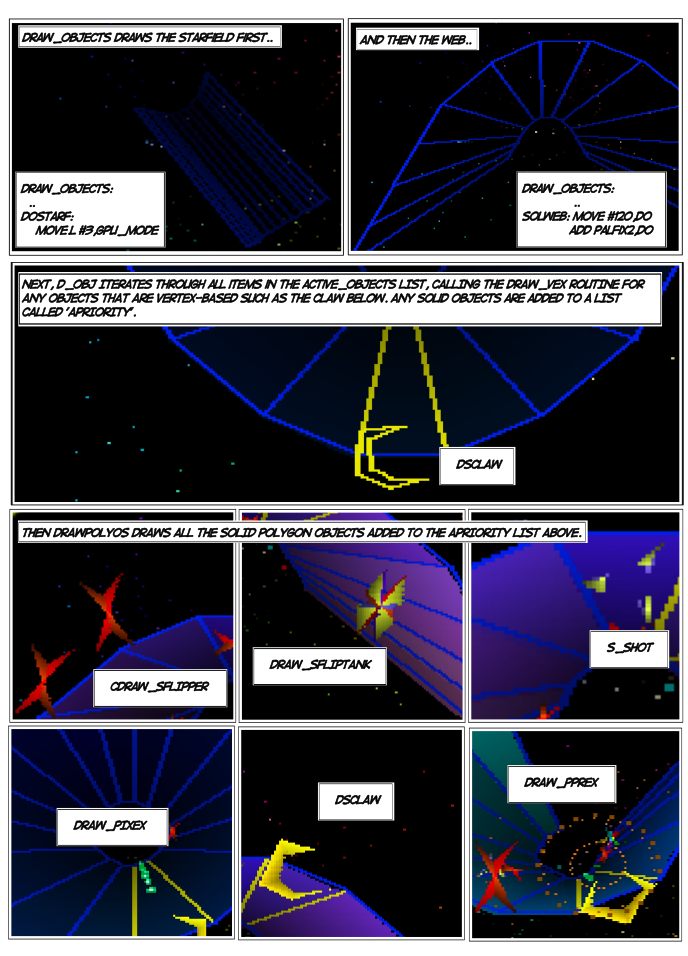
\includegraphics[width=13.7cm]{src/mainloop/mainloop-draw_objects-comic.png}%
\end{figure}

\begin{lstlisting}[escapechar=\%]
gwb:    move.l vp_x,d3         ; Stash player's X viewpoint in d3.
        move.l vp_y,d4         ; Stash player's Y viewpoint in d4.
        move.l vp_z,d5         ; Stash player's Z viewpoint in d5.
    
solweb: move #120,d0           ; Set register d0 to 120.
        add palfix2,d0         ; Adjust for PAL screens if required.
        and.l #$ff,d0          ; Keep it between 0 and 255
        move.l d0,ycent        ; Store result as the Y centre.
        tst l_solidweb         ; Are we drawing a solid web?
        beq vweb               ; If not, skip to vweb. 
        cmp #1,webcol          ; Drawing a transparent web?
        beq vweb               ; If so, skip to vweb.
        lea _web,a6            ; Load the web data structure to a6.
        tst 34(a6)             ; Is the web active? 
        beq n_wb               ; If not, skip 
        lea in_buf,a0          ; Point our GPU RAM input buffer at a0.
        move.l 46(a6),d0       ; Get ppinter to web data structure.
        move.l d0,(a0)         ; Store it in the in_buf.
        move.l 4(a6),d0        ; Get the source X position.
        sub.l d3,d0            ; Subtract vp_x, player's X viewpoint.
        move.l d0,4(a0)        ; Store it in the in_buf.
        move.l 8(a6),d0        ; Get the object's Y position.
        sub.l d4,d0            ; Subtract vp_y, player's Y viewpoint.
        move.l d0,8(a0)        ; Store it in the in_buf.
        move.l 12(a6),d0       ; Get the object's Z position.
        sub.l d5,d0            ; Subtract vp_z, player's Z viewpoint.
        bmi n_wb               ; If web not visible to player, skip.
        move.l d0,12(a0)       ; Store it in the in_buf.
        move l_solidweb,d0     ; Get X centre of Web. 
        and.l #$ff,d0          ; Keep it between 0 and 255
        move.l d0,16(a0)       ; Store it in the in_buf.
        move 28(a6),d0         ; Get Y centre of web.
        and.l #$ff,d0          ; Keep it between 0 and 255
        move.l d0,24(a0)       ; Store it in the in_buf.
        move frames,d0         ; Stash the frame count in d0.
        and.l #$ff,d0          ; Keep it between 0 and 255
        move.l d0,28(a0)       ; Store it as the rotation angle in in_buf.
        move.l #w16col,32(a0)  ; Store the rotation table in in_buf.
        move.l #0,gpu_mode     ; Select the web3d shader in donky.gas.
        lea equine2,a0         ; Load the GPU module in donky.gas.
        jsr gpurun             ; Run the selected GPU module.
        jsr gpuwait            ; Wait for the GPU to finish.
        jsr WaitBlit           ; Wait for the blitter to finish.
    
\end{lstlisting}
You may note at the end that we call a routine called \icode{WaitBlit}. This is because in addition to computing the
polygons that make up the 3D web, the GPU also 'blits' or writes its results to a buffer that will ultimately be used
by the Object Processor to write the pixels to the screen. It is this dual operation that caused Minter a headache
when attempting it from within the vertical sync interrupt. (My own suspicion is that there just wasn't enough time in the
interrupt to do everything he wanted on the GPU and Blitter - so moving it here to the mainloop ensured that it would only
be done opportunistically and at the risk of missing a frame every now and then.)

But there is more to Tempest 2000 than starfields and webs so there must be plenty of other things being drawn in here too.
At first it is not easy to see where though. The next section of the \icode{draw\_objects} routine is cryptic at best 
but on close inspection does contain some clues. As elsewhere, I've added comments to assist understanding:

\begin{lstlisting}
        ; Finished drawing the web, now for the activeobjects.
n_wb:   move.l activeobjects,a6    ; Store activeobjects pointer in a6.
        bsr d_obj             ; Run the d_obj routine below.
        bra odend             ; And go to end when done.
    
        ; A loop for processing everything in 'activeobjects'.
d_obj:  cmpa.l #-1,a6         ; Have we reached the end of activeobjects?
        beq oooend            ; If yes, skip to end.
        move 50(a6),d0        ; Is the object marked for deletion?
        beq no_unlink         ; If not, skip to no_unlink and draw it.
    
        ; This verbose section up until no_unlink is concerned entirely
        ; with deleting the dead object from the activeobjects list.
        move.l 56(a6),d1      ; Get address of previous object.
        bmi tlink             ; If none, skip to tlink.
        move.l d1,a5          ; Move previous object to a5.
        move.l 60(a6),60(a5)  ; Make it invisible to the vsync interrupt.
    
tlink:  move #-1,50(a6)       ; Mark the object for deletion.
        move.l 60(a6),-(a7)   ; Stash address of next object in the stack.
        move d0,-(a7)         ; Stash d0 in the stack.
        move.l a6,a0          ; Store the object (a6) in a0.
        move 32(a6),-(a7)     ; Stash the player ownership tag.
        move (a7)+,d1         ; Store the player ownership tag in d1.
        move (a7)+,d0         ; Store the object type in d0.
        lea uls,a1            ; Point a1 at uls.
        asl #2,d0             ; Multiply it by 4.
        move.l -4(a1,d0.w),a1 ; Use d0 as an index in to 'uls'.
        jmp (a1)              ; Jump to one of afinc, ashinc, pshinc.
    
        ; Object specific unlinking/deletion routines
uls:    dc.l afinc,ashinc,pshinc
    
        ; For unlinking a player shot object.
pshinc: tst d1                ; Is it owned by a player?
        beq ulsh1             ; If not, skip to ulsh1.
        add #1,shots+2        ; Make another shot available to player 1.
ulo:    move #1,locked        ; Lock activeobjects while we delete from it.
        bsr unlinkobject      ; Remove the object from activeobjects.
        clr locked            ; Unlock the activeobjects list again.
        bra nxt_o             ; Finished deleting, go the the next object.
ulsh1:  add #1,shots          ; Make another shot available to player 2.
        bra ulo
    
        ; For unlinking an enemy shot object.
ashinc: add #1,ashots         ; Make another shot available to enemies.
    
        ; For unlinking a default object.
afinc:  add #1,afree          ; Make slot available for a new activeobject.
        bra ulo
    
        ; Actually draw the object.
        ; No need to remove the object, just draw it.
no_unlink:
        lea draw_vex,a0       ; Get our table of draw routines.
        move 34(a6),d0        ; Is this object smaller than a pixel?
        bpl notpxl            ; If not, go to notpxl.
        move.l #draw_pel,a0   ; Use draw_pex for pixel-size objects.
        bra apal              ; Jump to the draw call.
notpxl: asl #2,d0             ; Multiply the val in d0 by 4.
        move.l 0(a0,d0.w),a0  ; Use it as an index into draw_vex.
apal:   move.l 60(a6),-(a7)   ; Store the index of next object in a7.
        jsr (a0)              ; But first call the routine in draw_vex.
        jsr gpuwait           ; Wait for the GPU to finish.
nxt_o:  clr locked            ; Clear 'locked' just in case.
nxt_ob: move.l (a7)+,a6       ; Put the index of next object back in a6.
        bra d_obj             ; Go to the next object.
\end{lstlisting}

This part of the \icode{draw\_objects} routine is concerned with processing a linked list called
\icode{activeobjects} using a loop that runs from \icode{d\_obj} to \icode{bra d\_obj} on the
last line. This \icode{activeobjects} list contains the detail for all objects that
are active on the screen and require drawing by the GPU/Blitter. Some of the original (but sparse)
code comments added by Minter suggest that this was initially conceived as a list for managing just
the player and enemy bullets but it expanded over time. 

Each object in the \icode{activeobjects} list has the following structure:

\begin{figure}[H]
  {
    \setlength{\tabcolsep}{3.0pt}
    \setlength\cmidrulewidth{\heavyrulewidth} % Make cmidrule = 
    \begin{adjustbox}{width=6cm,center}

      \begin{tabular}{lll}
        \toprule
        Bytes & Description\\
        \midrule
        0-4 & Vector Object or Solid Object \\ 
        4-8 &  X \\
        8-12 &  Y \\
        12-16 &  Z \\
        16-20 & Position on web.\\
        20-24 & Velocity \\
        24-28 & Acceleration  \& XY orientation \\
        28-30 & XZ Orientation \& XZ orientation  \\
        30-32 & Y Rotation \\
        32-34 & Z Rotation \\
        34-36 & Index into draw routine in \icode{draw\_vex}.\\
        36-38 & Start address of pixel data. \& Delta Z \\
        38-40 & Y \& Colour change value\\
        40-42 & Colour \\
        42-44 & Scale factor \\
        \bottomrule
      \end{tabular}
    \end{adjustbox}
  }\caption*{The structure of objects in \icode{activeobjects}.}
\end{figure}

\begin{figure}[H]
  {
    \setlength{\tabcolsep}{3.0pt}
    \setlength\cmidrulewidth{\heavyrulewidth} % Make cmidrule = 
    \begin{adjustbox}{width=6cm,center}

      \begin{tabular}{lll}
        \toprule
        Bytes & Description\\
        \midrule
        44-46 & Mode to climb, descend or cross rail \\
        46-48 & Size of Pixel Data  \& Duration.\\
        48-50 & Fire Timer \\
        50-52 & Marked for deletion \\
        52-54 & Whether an enemy or not. \\
        54-56 & Object Type \\
        56-60 & Address of Previous Object \\
        60-64 & Address of Next Object \\
        \bottomrule
      \end{tabular}
    \end{adjustbox}
  }\caption*{The structure of objects in \icode{activeobjects} continued.}
\end{figure}

So in the 64 bytes of each object we cover quite a bit of ground. There is colour, co-ordinate, motion, and orientation
information. There's also detail that defines the behaviour of the object and most immediately relevant to what
we are looking at here, an index into the draw routine to use for the object at bytes 34-36.

This index is a value that references the routine given at the appropriate position in the \icode{draw\_vex} array:
\begin{lstlisting}
draw_vex: 
   dc.l rrts,draw,draw_z,draw_vxc,draw_spike,draw_pixex,draw_mpixex,draw_oneup,draw_pel,changex
   dc.l draw_pring,draw_prex,dxshot,drawsphere,draw_fw,dmpix,dsclaw,dsclaw2
\end{lstlisting}

The draw routine can vary depending on the type of object. There's a distinct treatment of vector object and objects
that are solid polygons. Vector objects require the least work and if the header in bytes 0-4 indicates that it requires
vector drawing only (for example the player's claw) then a vector draw in the GPU will suffice. The \icode{draw} routine
in the second item in \icode{draw\_vex} is the base routine for deciding whether a vector draw is sufficient or not, and
most of the other routines make use of it in addition to the object-specific detail they manage:

\begin{lstlisting}
; *******************************************************************
; draw
; The 'base' draw routine when processing 'activeobjects'. If a 'vector'
; draw is good enough, we just do that. Otherwise we add the object to the
; 'apriority' list for processing by 'drawpolyos'. The object to draw is
; passed in the a6 register.
; *******************************************************************
draw:
        move.l a6,oopss     ; Stash the header.
        ; If the header contains a negative value it's an index into the
        ; 'solids' list, otherwise it's the address of the vector data
        ; object we can draw directly with the gpu.
        move.l (a6),d0      ; Is the header value greater than zero?
        bpl vector          ; If yes, then a vector draw will suffice.
    
        ; Otherwise we need to do add this object to the 'apriority'
        ; list so that it can be drawn as a solid polygon.
        ; The 'apriority' list stores objects in the descending order
        ; of their Z co-ordinate. This ensures that nearer objects are
        ; painted in front of objects that are further away or 'behind' them.
        move.l fpriority,a0 ; Get a free priority object
        move.l a6,(a0)      ; Store the object we're drawing in a0.
        move.l 12(a6),d0    ; Put the object's Z value in d0.
        move.l d0,12(a0)    ; Put z in prior object
        move.l apriority,a1 ; Store pointer to apriority in a1.
        move.l a1,a2        ; And also in a2.

        ; Loop through the apriority list looking for the right place
        ; to store the current object.
chklp:  cmp.l #-1,a1        ; Is the list empty?
        bne prio1           ; If not, skip to prio1 otherwise..
        bra insertprior     ; Insert the object in the apriority list.
    
prio1:  cmp.l 12(a1),d0     ; Check Z value of object in list against ours. 
        bge insertprior     ; If it's less, then insert our object here.
        move.l a1,a2        ; Otherwise stash that object.
        move.l 8(a1),a1     ; And store the next object in a1.
        bra chklp           ; loop until list end or next object in front of us
        rts                 ; return with object at right place in the list
\end{lstlisting}

Reading through the above we can see that if a \icode{vector} draw won't do the job then the object gets
added to a list called \icode{apriority} and nothing else is done with it for now. So what we are doing in our
\icode{d\_obj} loop is a first pass through the \icode{activeobjects} list, with any items on the list that 
require attention to the order in which they are painted, passed off to the \icode{apriority} list. Notice
that we don't mutate or update the objects in any way, we simply pass them over so the structure of the objects
we described above remains unchanged. What we're doing with this list is ensuring that the Z co-ordinate position
of each object is respected, so that objects nearer the viewer are painted after the ones that are further away. This
ensures that nearer objects are painted over further objects.

Once we have finished this first run through the \icode{activeobjects} list our next order of business
is to process the \icode{apriority} list we've populated. This is done in \icode{drawpolyos} which we
call right after we've finished with our first pass of \icode{activeobjects}. 

\begin{lstlisting}
        ; We've finished our first pass of activeobjects.
odend:
        bsr showscore     ; Show the score.
        ; In Tempest Classic mode we don't need solid polygons.
        tst blanka        ; Are we doing solid polygons?
        beq odvec         ; If not, skip.
        bsr drawpolyos    ; if we are, draw them.
\end{lstlisting}

Drawing our polygons happens below. We iterate through the 'apriority' list, deleting items in it
as we go, and calling the object-specific draw routine for each to render them to the screen.


\begin{lstlisting}
; Routine for drawing all solid polygons.
; Process each object in the 'apriority' list. We remove each item after
; processing.The draw routine for each item is given by its index into
; the 'solids' array.
drawpolyos:
        move.l #192,xcent   ; Set 192 as X centre.
        move.l #120,d6      ; Set 120 as Y centre.
        add palfix2,d6      ; Adjust for PAL if necessary.
        move.l d6,ycent     ; Store it as Y centre.
        move.l apriority,a0 ; Get our 'apriority' list.

dpoloop:cmp.l #-1,a0        ; Have we reached the end of the list?
        beq rrts            ; If yes, bail out now.
        move.l (a0),a6      ; Get the index to 'solids'
        move.l (a6),d0      ; Store it in d0.
        move.l a0,-(a7)     ; Stash our current position in the list.
        bsr podraw          ; Go do object type draw
        jsr gpuwait         ; wait for gpu
        move.l (a7)+,a0     ; Get our current position in the list
        move.l 8(a0),-(a7)  ; Get the next position in the list
        bsr unlinkprior     ; Delete the current object.
        move.l (a7)+,a0     ; Move to the next position in the list.
        bra dpoloop         ; Loop until all objects drawn and unlinked
 
podraw: move.l #9,d4        ; Set X centre as 9.
        move.l #9,d5        ; Set Y centre as 9.
        neg d0              ; Negate d0.
        lea solids,a4       ; Get the 'solids' list.
        lsl #2,d0           ; Multiply our index by 2.
        move.l 0(a4,d0.w),a0  ; Get the draw routine address from 'solids'.
        move.l 4(a6),d2     ; Get the X position from our object.
        sub.l vp_x,d2       ; Subtract our X viewpoint.
        move.l 8(a6),d3     ; Get the Y position from our object.
        sub.l vp_y,d3       ; Subtract our Y viewpoint.
        move.l 12(a6),d1    ; Get the Z position from our object.
        sub.l vp_z,d1       ; Subtract our X viewpoint.
        bmi rrts            ; Skip if not visible.
        move 28(a6),d0      ; Get orientation of object.
        and.l #$ff,d0       ; Use only the least significant bytes.
        ; Because we jmp to the draw routine, when it returns, execution
        ; will go back to the caller of 'podraw' in dpoloop above.
        jmp (a0)            ; Call the object's draw routine.
\end{lstlisting}

You'll notice that we're choosing an object draw routine from something
called a \icode{solids} list. This is a list of draw routines and each
object contains an index into this list for its specific routine. For example,
a flipper object will have an index of \icode{1} pointing ot the \icode{cdraw\_sflipper}
routine in \icode{solids}:

\begin{lstlisting}
solids: 
        dc.l rrts,cdraw_sflipper,draw_sfliptank,s_shot,draw_sfuseball
        dc.l draw_spulsar,draw_sfusetank,ringbull,draw_spulstank
        dc.l draw_pixex,draw_pup1,draw_gate,draw_h2hclaw,draw_mirr
        dc.l draw_h2hshot,draw_h2hgen,dxshot,draw_pprex,draw_h2hball
        dc.l draw_blueflip,ringbull,supf1,supf2,draw_beast,dr_beast3
        dc.l dr_beast2,draw_adroid            
\end{lstlisting}

\section*{creating and updating objects}
Drawing objects is all very well, but first we must create them. And once we've
created them, we need to keep updating them. Enemies, bullets and even players
have a habit of moving around. 

As we mentioned previously, initially Minter tried doing both the drawing and the
updating of objects in the same place, during the vertical sync interrupt that
occurs when the Jaguar has finished painting a frame. Since it turned out there
wasn't enough time to do both in the short interval that the vertical sync interrupt
allows, he had to move the drawing work to \icode{mainloop}. So when we first look at
the code that remains in the vertical sync interrupt routine (which is called
\icode{Frame}), we find that is concerned almost everything except keeping 
the \icode{activeobjects} list fresh up-to-date. There is a lot of time spent
on managing double-buffering, playing sounds, checking for player input and even some
redundant logic for checking the rotary controller.

The updating of objects in the \icode{activeobjects} list, and the creation of new ones,
is instead buried in this little paragaph:
\begin{lstlisting}
doframe:
        move.l routine,a0  ; Stash the current 'routine' in a0.
        jsr (a0)           ; Run it.
\end{lstlisting}

The routine that \icode{routine} points to is updated regularly to reflect the current
state of the game. There are a number of different routines it can point to, some of 
them more self-explanatory than others.
\begin{lstlisting}
;  rrts, pauson, pausing, budb, pausoff, paws, zoom1, zoomto,
;  waitfor, zprev, znext, zshow, oselector, seldb, tunrun, text_o_run,
;  m7run, vicrun, failcount, viccount, txen, tgoto, rotate_web,
;  zoom3, zap_player, take_me_to_your_leader, snatch_it_away,
;  moveclaw, zoom2
\end{lstlisting}

\begin{figure}[H]
      \centering
      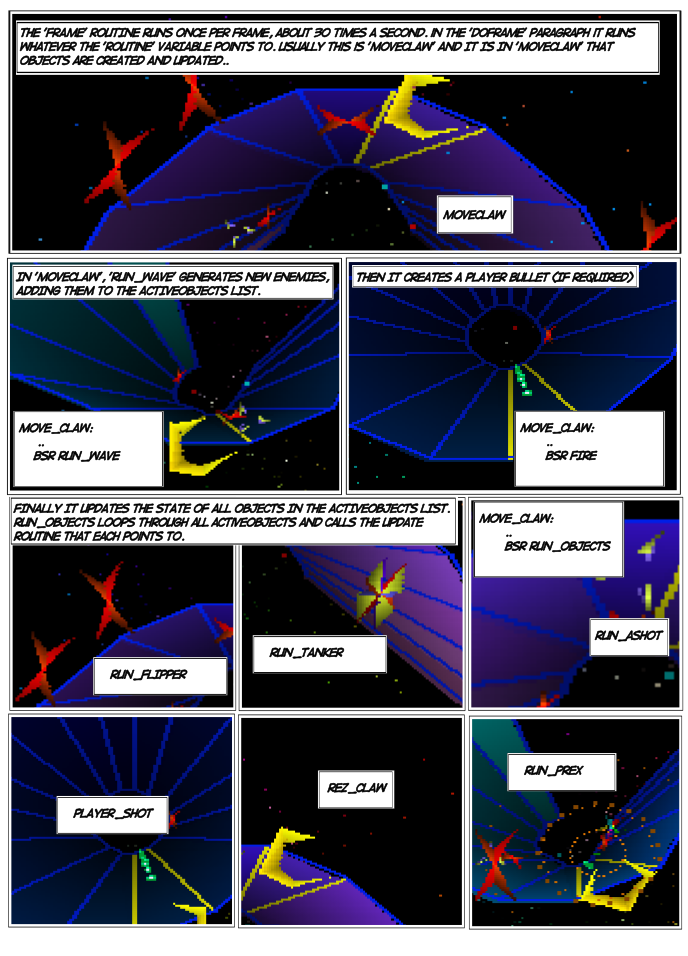
\includegraphics[width=13.7cm]{src/mainloop/mainloop-run_objects-comic.png}%
\end{figure}

Every now and then, in fact more often than not, \icode{routine} will point to a routine
buried in the list above called \icode{moveclaw}. Despite its name, it is \icode{moveclaw} that looks after
the bits we're interested in.


\begin{lstlisting}
; *******************************************************************
; Despite its name this routine updates the state of most active game
; objects in addition to just the claw.
; Move the claw, generate waves, update some objects.
; run_wave: Manages all enemies for this frame, including generating
;           new ones.
; *******************************************************************
moveclaw:
        bsr vp_xform               ; do dynamic vp
        tst h2h                    ; Are we playing a head-to-head game?
        bne h2hrun                 ; If yes, go to h2hrun.
        bsr run_wave               ; Otherwise run the wave generater!
        tst chenable               ; Is cheating enabled?
        beq nofire                 ; If not, skip to nofire.

        ; Check if the Option button cheat was selected.
        cmp #-2,wave_tim           ; Is the wave finished already?
        beq nofire                 ; If so, skip to nofire.
        btst.b #1,pad_now+2        ; Is the option button pressed? 
        beq noptcheat              ; If not skip to noptcheat.
        ; Otherwise cheat, get more points and go to next level.
        jsr douttah                ; Add points and go to next level.
        bra nofire                 ; Update objects and clean up.
    
        ; Another cheat, pressing 6 lets us warp to next level.
noptcheat:
        move.l pad_now,d0          ; Store pressed buttons in d0.
        and.l #six,d0              ; Is the 6 button pressed?
        beq nofire                 ; If not skip to nofire.
        ; Otherwise the cheat has been selected.
        jsr swarp                  ; Warp to next level!

        ; Fire bullets, update all activeobjects, and update
        ; the player's viewpoint.
nofire: bsr fire                   ; Fire a bullet if necessary.
        ; The main routine for updating the state of all the active
        ; objects in the game and the overall game state.
        bsr run_objects            ; Update active objects
        bsr vp_set                 ; Update camera viewpoint.
        rts
\end{lstlisting}

The key elements in here are \icode{run\_wave} near the top, and \icode{run\_objects}
near the bottom. The first creates new enemies if required, while the second does
the important job of updating all the active objects in the game such as the flippers,
bullets, and the player's claw itself. The illustration opposite hopefully gives you a
general idea.

Both of these routines are quite substantial, so I'm not going to list them in full. Instead
we're going to concentrate on the section in \icode{run\_objects} that deals with updating
the state of objects.

\begin{lstlisting}
        ; Iterate through the activobjects list in a6 and run
        ; the appropriate routine in 'run_vex' for each object.
r_obj:  cmpa.l #-1,a6        ; Are we at the end of the activeobjects list?
        beq r_end            ; If so, clean up and exit.
        tst 50(a6)           ; Is the object marked for deletion?
        bmi r_end1           ; If so, exit and clean up.
        lea run_vex,a0       ; Store run_vex in a0
        ...
        move 54(a6),d0       ; Put the object type in d0.
        ..
r_o1:   asl #2,d0            ; Multiply it by 4.
        ; Put address of next object in stack in case this one is unlinked.
        move.l 60(a6),-(a7)  ; Push address of next object to stack. 
        move.l 0(a0,d0.w),a0 ; Use d0 as index into run_vex.
        tst 52(a6)           ; Is the object an 'Enemy'?
        beq zokk             ; (don't count player bulls)
        bmi zokk             ; (or claw VULNERABLE flags)
        cmp 12(a6),d6        ; Check against previous nearest
        blt gokk             ; If less, don't swap.
        swap d6              ; Swap position of first 2 bytes with last 2.
        move 16(a6),d6       ; get nearest one's Lane #
        swap d6              ; Swap position of first 2 bytes with last 2.
        move 12(a6),d6       ; make this z nearest
gokk:   cmp 12(a6),d7        ; Is the z value the nearest so far?
        bgt zokk             ; If not, skip to zokk, otherwise..
        move 12(a6),d7       ; Store it as the new nearest.
zokk:   movem.l d6-d7,-(a7)  ; Stash values in the stack.
        move #3,diag         ; Update our diagnostic bytes to step 3..
        move.l a0,diag+4     ; .. used for debugging where we are..
        move.l a6,diag+8     ; .. in this routine.
        tst locked           ; Are we alreadyadding stuff to activeobjects?
        bne hack             ; If so, don't run the object update routine.
        jsr (a0)             ; Run the update routine selected from run_vex.
hack:   movem.l (a7)+,d6-d7  ; retrieve furthest-z
        move.l (a7)+,a6      ; Put the next object in a6.
        move #4,diag         ; Update our diagnostic bytes to step 4..
        move.l a6,diag+12    ; Store the object pointer in diagnostic bytes.
        bra r_obj            ; Move to the next object in activeobjects.
\end{lstlisting}

There is some accounting in here to ensure that the z position of the objects are updated
depending on their current position relative to each other, but the main business is towards
the very end where we call the appropriate update routine for the object given by its index
into the \icode{run\_vex} list. This is stored at at byte 54 of the object and will tell
us which of the routines in \icode{run\_vex} to use. For example a flipper object will
have an index of \icode{2} pointing to \icode{run\_flipper}. A player bullet will have an
index of \icode{1}, pointing to \icode{player\_shot}.

\clearpage

\begin{lstlisting}
run_vex:
    dc.l rrts,player_shot,run_flipper,run_zap,kill_shot,run_tanker,run_spike
    dc.l run_spiker,run_ashot,run_fuseball,blowaway,run_pulsar,oblow
    dc.l go_downc,go_downf,claw_con2,claw_con1,rez_claw,czoom1,czoom2
    dc.l pzap,rundroid,dc.l run_pixex,run_pspark,run_prex,run_pup,xshot
    dc.l run_gate,xr_pixex,run_fw,run_h2hclaw,run_mirr,run_h2hshot
    dc.l run_h2hgen,run_h2hball,oblow2,rumirr,refsht,refsht2,run_adroid
\end{lstlisting}

In fact \icode{player\_shot} is a good example of how straightforward these
object update routines can be. As we can see below, it consists simply of
rotating the object, updating its color to make if flash, incrementing its
Z position to move it along the web, and finally deciding whether it has
reached the end of its life and should be deleted.

\begin{lstlisting}
; *******************************************************************
; player_shot: move a standard Tempest player's shot
; *******************************************************************
player_shot:
        add #8,28(a6)        ; Increment the XZ orientation to spin it.
        add.b #$30,41(a6)    ; Increment the color value to make it flash.
        move.l shotspeed,d0  ; Put shot speed in d0.
        ; Increment the z position by the shot speed, so that
        ; it moves along the web.
        add.l d0,12(a6)      ; Increment the z position.
        cmp #webz+80,12(a6)  ; Check if it has reached the end of the web.
        blt rrts             ; If not, we're done.
        move.l 24(a6),a1     ; Otherwise, point a1 at the XY orientation..
        clr.l (a1)           ; .. and clear it.
        move.l a6,a0         ; Point a0 at the object data.
        move #3,50(a6)       ; Mark the object for deletion.
        rts
\end{lstlisting}
